
\section{Diffusion Probabilistic models} \label{appendix:diffusion}
Given i.i.d. samples $\{\mathbf{x}_{0} \in \mathbb{R}^{D}\}$ from an unknown data distribution $p_{data}(\mathbf{x}_{0})$. In this section, we introduce the theory of diffusion probabilistic model~\cite{ho2020denoising,lam2022bddm,song2020denoising,song2020score}. First, we present diffusion and reverse process given by denoising diffusion probabilistic models (DDPMs), which could be used to learn a model distribution $p_{\theta}(\mathbf{x}_{0})$ that approximates $p_{data}(\mathbf{x}_{0})$. Secondly, we introduce the recently proposed bilateral denoising diffusion models (BDDMs) and its tighter evidence lower bound (ELBO) for acceleration. 

\paragraph{Diffusion process}  Similar as previous work~\cite{ho2020denoising,lam2022bddm,song2020denoising}, we define the data distribution as $q(\mathbf{x}_{0})$. The diffusion process is defined by a fixed Markov chain from data $x_0$ to the latent variable $x_T$:
\begin{align}
q(\vx_{1},\cdots,\vx_T|x_0) = \prod_{t=1}^T q(\vx_t|\vx_{t-1}),
\quad\ \ 
\end{align}

For a small positive constant $\beta_t$, a small Gaussian noise is added from $x_{t}$ to the distribution of $x_{t-1}$ under the function of $q(x_t|x_{t-1})$.

The whole process gradually converts data $x_0$ to whitened latents $x_T$ according to the fixed noise schedule $\beta_1,\cdots,\beta_T$.
\begin{align}
q(\vx_t|\vx_{t-1}) := \gN(\vx_t;\sqrt{1-\beta_t}\vx_{t-1},\beta_t I)
\end{align}

Efficient training is optimizing a random term of $t$ with stochastic gradient descent: 

\begin{align}
    \label{eq: score_loss}
    \gL_{\theta} = \left\lVert \beps_\theta\left(\alpha_t\rvx_{0}+\sqrt{1-\alpha_t^2}\beps\right)-\beps\right\rVert_2^2, \beps\sim\gN(\vzero, \mI)
\end{align}


\paragraph{Reverse process}  Unlike the diffusion process, reverse process is to recover samples from Gaussian noises. The reverse process is a Markov chain from $x_T$ to $x_0$ parameterized by shared $\theta$:
\begin{align}
p_{\theta}(\vx_0,\cdots,\vx_{T-1}|x_T)=\prod_{t=1}^T p_{\theta}(\vx_{t-1}|\vx_t),
\end{align}

where each iteration eliminate the Gaussian noise added in the diffusion process:
\begin{align}
    p(\vx_t|\vx_{t-1}) := \mathcal{N}(\vx_{t-1};\mu_{\theta}(\vx_t,t), \sigma_{\theta}(\vx_t,t)^2I)
\end{align}

\paragraph{Acceration} 
Recently, Bilateral denoising diffusion models (BDDMs)~\cite{lam2022bddm} demonstrates its tighter evidence lower bound (ELBO) for noise schedule prediction. Given a leaned diffusion network $\theta$, a scheduling network $\phi$ could be applied in reducing the gap between the proposed surrogate objective. To be more specific, instead of using the fixed one in diffusion process, a much more efficient N-step noise schedule (i.e., $\hat{\beta}$) could be derived by the well-leaned noise scheduling network $\phi$. The noise schedule could be applied in reverse process, making it possible to explicitly trade-off between inference computation and output quality in one model. 

For learning the noise schedule predictor $\phi$, we apply the loss function as a KL divergence term between the forward and the reverse distribution:
\begin{equation} \label{eq: noise_loss}
    \resizebox{.99\linewidth}{!}{$
    \gL_{\phi}= \frac{1}{2(1-\beta_{t}-\alpha_{t}^{2})}\|\sqrt{1-\alpha_{t}^{2}} \beps_{t}-\frac{\beta_{t}}{\sqrt{1-\alpha_{t}^{2}}} \beps_{\theta}(\vx_{t}, \alpha_{t})\|_{2}^{2} +C_{t}
    $}
\end{equation}
where $C_{t} =\frac{1}{4} \log \frac{1-\alpha_{t}^{2}}{\beta_{t}}+\frac{D}{2}(\frac{\beta_{t}}{1-\alpha_{t}^{2}}-1)$ is a constant that can be ignored during training.


\section{Model Architectures} \label{appendix:arch}
\subsection{FastDiff} 
\label{appendix:arch_refime} \label{appendix:noise_predictor}


As illustrated in Table \ref{tab:hyperparameters}, we list the hyper-parameters of FastDiff. We further visualize the detailed architectures of the noise predictor and DBlock in the refinement model in Figure~\ref{fig:noise_predictor}.

\begin{table}[h]
\centering
\begin{minipage}[t]{\linewidth}
\centering
\begin{tabular}{l|l}
\hline
\textbf{Hyperparameter}               &  \textbf{FastDiff}  \\
\toprule
\textbf{Refinement Model $\theta$}    &               \\
DBlock Hidden Channels                 &     32     \\ 
DBlock Downsample Ratios               &  [4, 8, 8]           \\ 
Diffusion UBlock Hidden Channels      &    32          \\
Diffusion UBlock Upsample Ratios       &    [8, 8, 4]    \\
Time-aware LVC layers Each Block       &      4         \\
Time-aware LVC layers Kernel Size      &      256       \\
Diffusion Kernel Predictor Hidden Channels   &       64   \\  
Diffusion Kernel Predictor Kernel Size  &      3       \\
Diffusion Embedding Input Channels      &      128     \\
Diffusion Embedding Output Channels     &      512     \\
Use Weight Norm                         &      True          \\
\midrule
Total Number of Parameters             &           13M	         \\ 
\midrule
\textbf{Noise Predictor $\phi$}      &               \\
Window Length                       &  8 Samples             \\
Segment Size                        &  64             \\
Number of GALR Blocks               &  2             \\
GALR Blocks Hidden Channels         &  128             \\
\midrule
Total Number of Parameters          &   0.5M         \\ 
\bottomrule
\end{tabular}
\caption{Architecture hyperparameters of FastDiff.}
\label{tab:hyperparameters}
\end{minipage}
\end{table}




% GALR is a speech separation neural network for efficient noise prediction $\phi$. 

% Following the configuration from previous work, we used a window length of 8 samples for encoding, a segment size of 64 for segmentation and only two GALR blocks of 128 hidden dimensions.



\begin{figure*}
    \vspace{-8mm}
    \centering
    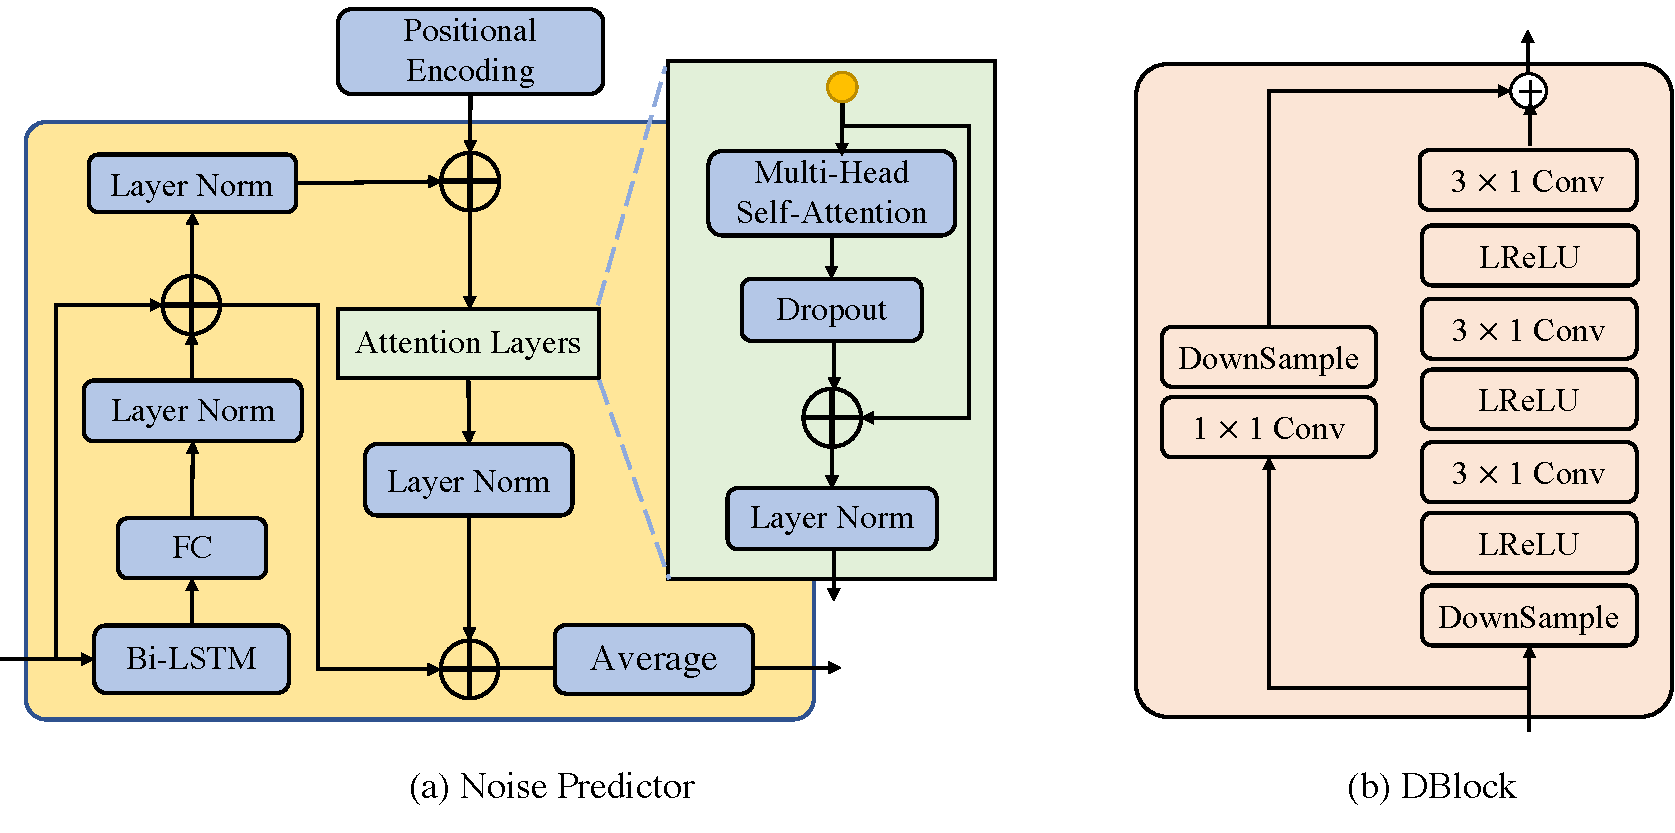
\includegraphics[width=0.6\textwidth,trim={1.0cm 0cm 1.0cm 0cm}]{Figures/arch2.pdf}
    \vspace{-3mm}
   \caption{The details of network architectures. Left: The GALR-block based noise predictor $\phi$. Right: DBlock in FastDiff $\theta$} 
    \label{fig:noise_predictor}
  \end{figure*}

\subsection{FastDiff-TTS} \label{appendix:fastDiff_tts}
In this section, we list the model hyper-parameters of FastDiff-TTS in Table \ref{tab:hyperparameters}.
% The hidden sizes of the self-attention and 1D convolution in each feed-forward Transformer block are all set to 256. The number of attention heads and hidden channel are set to 2, 256, respectively. In the duration and pitch predictor, the kernel sizes of the 1D-convolution are set to 3. 

\begin{table}[H]
    \begin{minipage}[t]{\linewidth}
        \centering
        \begin{tabular}{l|l}
        \hline
        \textbf{Hyperparameter}               &  \textbf{FastDiff-TTS}  \\
        \toprule
        Phoneme Embedding Dimension             &  256                   \\ 
        Pre-net Layers                          &      3                         \\ 
        Pre-net Hidden                        &     256                          \\ 
        Encoder Layers                         &      4                       \\ 
        Encoder Hidden                         &      256                         \\
        Encoder Conv1D Kernel                  &       9                         \\ 
        Encoder Conv1D Filter Size             &      1024                         \\
        Encoder Attention Heads                &      2                       \\
        Encoder/Decoder Dropout                &      0.1                     \\
        Variance Predictor Conv1D Kernel       &  3                          \\ 
        Variance Predictor Conv1D Filter Size  &  256                      \\ 
        Variance Predictor Dropout              &   0.5                 \\ 
        FastDiff wave decoder               &   Follow Table~\ref{tab:hyperparameters}              \\ 
        \midrule
        Total Number of Parameters            &           40M	         \\
        \bottomrule
        \end{tabular}
        \caption{Architecture hyperparameters of FastDiff-TTS.}
        \label{tab:hyperparameters_tts}
        \end{minipage}
\end{table}

\section{Training, Noise scheduling and Inference details}  \label{appendix:Training}

\subsection{Diffusion hyperparameters} \label{appendix:noise_schedule}
We list the diffusion hyper-parameters of FastDiff and FastDiff/FastDiff-TTS in Table \ref{tab:apx_diffusionhyperparameters}. 


\begin{table}[h]
    \small
    \centering
    \begin{tabular}{l}
    \hline
    \textbf{Diffusion Hyperparameter}       \\
    \toprule 
    \textbf{Noise Scheduling}                \\
    $\tau = 200, \hat{\alpha_{t}} = 0.54, \hat{\beta_{t}} = 0.70, N = 4$                                            \\  
    \midrule
    \textbf{Training and Sampling}                            \\
    \textbf{Pre-defined (T = $1000$)}: \\ $\beta= \text{Linear} (1\times 10^{-4}, 0.005, 1000)$       \\
    \textbf{Grid Search ($T_m = 4$) derived}:  \\ $ \hat{\beta} = [3.6701e^{-7}, 1.7032e^{-5}, 7.908e^{-4}, 7.6146e^{-1}]$      \\
    \textbf{Noise Predictor ($T_m = 4$) derived}: \\ $ \hat{\beta} = [3.2176e^{-4}, 2.5743e^{-3}, 2.5376e^{-2}, 7.0414e^{-1}]$      \\
    \bottomrule
    \end{tabular}
    \caption{Diffusion hyperparameters of FastDiff and FastDiff-TTS.}
    \label{tab:apx_diffusionhyperparameters}
    \end{table}


\subsection{Noise Scheduling}  \label{appendix:algorithm}
Our noise scheduling algorithm mainly follows the bilateral denoising diffusion models~\cite{lam2022bddm}:
\begin{algorithm}[H]
    \centering
    \caption{Noise scheduling process}\label{alg: noise scheduling}
    \begin{algorithmic}[1]
    \STATE  \textbf{Input}: Pre-defined discrete $\beta$, trained refinement network $\theta$, hyperparameter $N, \hat{\alpha_{t}}, \hat{\beta_{t}}$.
    \FOR{$t=N,\cdots,2$}
    \STATE Sample $\vx_{t-1}\sim p_{\theta}(x_{t-1}|x_t)$
    \STATE  $\hat{\alpha}_{t-1}=\frac{\hat{\alpha}_{t}}{\sqrt{1-\hat{\beta}_{t}}}$
    \STATE  $\hat{\beta}_{t-1}=\min \left\{1-\hat{\alpha}_{t-1}^{2}, \hat{\beta}_{t}\right\} \phi\left(\hat{\boldsymbol{x}}_{t-1}\right)$
    \IF{$\hat{\beta}_{t-1}<\beta_{1}$}
    \RETURN $\hat{\beta}_{t}, \ldots, \hat{\beta}_{N}$
    \ENDIF
    \ENDFOR
    \RETURN $\hat{\beta}_{t}, \ldots, \hat{\beta}_{N}$
    \vspace{0.09em}
    \end{algorithmic}
\end{algorithm}

\subsection{Schedule Alignment}  \label{appendix:schedule_alignment}
Here we search and interpolate $\alpha_{s}$ between two training noise constants $l_{t}$ and $l_{t+1}$, enforcing $\alpha_{s}$ to get closed to $l_{t}$. In the end, we gain the well-mapped diffusion step $t_m$:

Firstly we compute the corresponding constants respective to diffusion and reverse process:
\begin{align}
    l_{t}=\prod_{i=1}^{t} \sqrt{1-\beta_{i}}, \quad \alpha_{s}=\prod_{i=1}^{s} \sqrt{1-\hat{\beta}_{i}}
\end{align}

Here we search and interpolate $\alpha_{s}$ between two training noise constants $l_{t}$ and $l_{t+1}$, enforcing $\alpha_{s}$ to get closed to $l_{t}$. In the end, we gain the well-mapped diffusion step $t_m$:

\begin{equation}\label{eq: aligned step}
    t_m = t + \frac{l_t-\alpha_s}{l_t-l_{t+1}} \quad \text{ if } \alpha_s\in[\ l_{t+1}, l_t\ ].
\end{equation}

Where integer $t$ represents a single pre-defined diffusion step, and $s$ presents a single step of noise schedule obtained through the scheduling process. Given these two schedules mentioned above, we could conduct schedule alignment and derive the floating-point $t_m$ for much more efficient reverse sampling.


\begin{figure*}
    \vspace{-2mm}
    \centering
    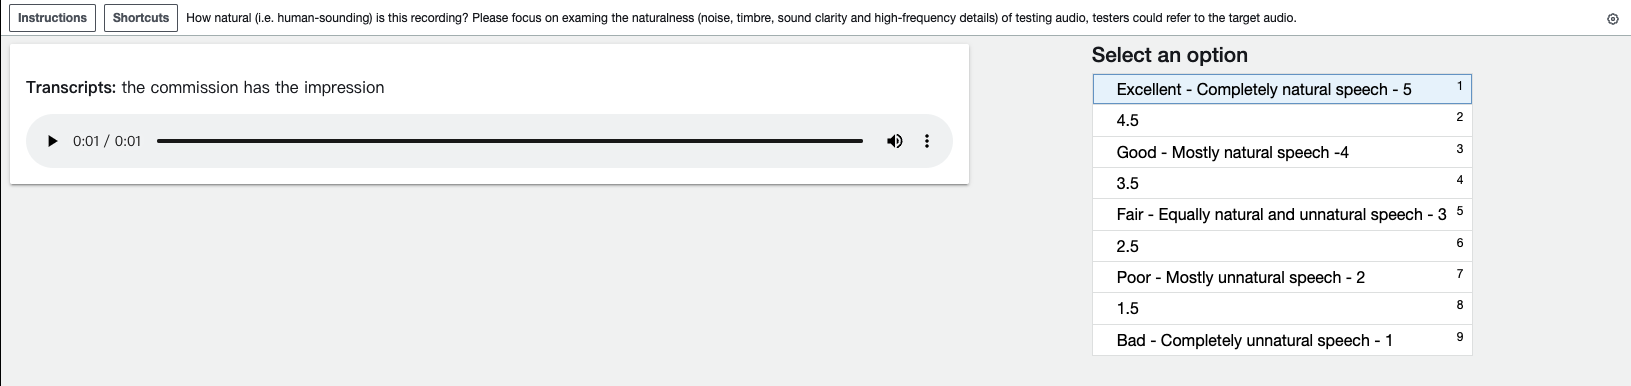
\includegraphics[width=0.8\textwidth]{Figures/mos_test.png}
    \vspace{-1mm}
   \caption{Screenshot of MOS testing.} 
    \label{fig:MOS}
  \end{figure*}
\section{Evaluation Matrix} \label{appendix:evaluation}

% \subsection{LS-MSE} Log-mel spectrogram mean squared error(LS-MSE) measure the consistency between the original waveform and the generated waveform in the Mel-frequency domain.

\subsection{PESQ and STOI} Perceptual evaluation of speech quality (PESQ)~\cite{rix2001perceptual} and The short-time objective intelligibility (STOI)~\cite{taal2010short} assesses the denoising quality for speech enhancement.

\subsection{NDB and JSD}
Number of Statistically-Different Bins (NDB) and Jensen-Shannon divergence (JSD). They measure diversity by 1) clustering the training data into several clusters, and 2) measuring how well the generated samples fit into those clusters. 


\subsection{Details in MOS Evaluation}



All our Mean Opinion Score (MOS) tests are crowd-sourced and conducted by native speakers. The scoring criteria has been included in Table~\ref{matrix:naturalness} for completeness. The samples are presented and rated one at a time by the testers, each tester is asked to evaluate the subjective naturalness of a sentence on a 1-5 Likert scale. The screenshots of instructions for testers are shown in Figure~\ref{fig:MOS}. We paid \$8 to participants hourly and totally spent about \$750 on participant compensation.

\begin{table}[ht]
  \vspace{-2mm}
 \centering
    \small
  \begin{tabular}{ccc}

  \toprule
  Rating & Naturalness & Definition                           \\
  \midrule
  1      & Bad        &  Very annoying and objectionable dist. \\
  2      & Poor       &  Annoying but not objectionable dist. \\
  3      & Fair       &  Perceptible and slightly annoying dist\\
  4      & Good       & Just perceptible but not annoying dist. \\
  5      & Excellent  & Imperceptible distortions\\
  \bottomrule
  \end{tabular}
  \caption{Ratings that have been used in evaluation of speech naturalness of synthetic and ground truth samples.}
  \label{matrix:naturalness}
  \vspace{-4mm}
  \end{table}


\section{Extension to Continuous Condition} \label{appendix:extension}

Our ablation study extends FastDiff to be conditioned on continuous noise levels and compares it to the basic model with the discrete condition. To be more specific, the FastDiff model conditioned on continuous noise levels does not require an additional schedule alignment process, which has a separated training and sampling procedure: 

\begin{algorithm}[H]
    \centering
    \caption{Training refinement network $\theta$ (Continuous Condition)}
    \begin{algorithmic}[1]
    \vspace{-0.1cm}
    \STATE \textbf{Input}: Pre-defined noise schedule $l$
    \REPEAT 
    \STATE Sample $\vx_{0} \sim q_{data}$, $\epsilon\sim\gN(0,I)$, and \quad $t\sim\mathrm{Unif}(\{1,\cdots,T\})$
    \STATE $\alpha_s \sim \operatorname{Uniform}\left(\alpha_{t-1}, \alpha_{t}\right)$
    \STATE $\vx_s = \alpha_{s} \vx_{0}+ \delta_s \epsilon$
    \STATE Take gradient descent steps on $\nabla_{\theta}\left\|\epsilon-\epsilon_{\theta}\left(\vx_s, \alpha_s\right)\right\|_{2}^{2}$ 
    \UNTIL{iterative refinement model $\theta$ converged}
    \vspace{0.09em}
    \end{algorithmic}
    \end{algorithm}

    \begin{algorithm}[H]
        \centering
        \caption{Sampling}
        \begin{algorithmic}[1]
        \STATE \textbf{Input}: Pre-defined $\beta, T$ and $\hat{\beta}$ derived in noise scheduling process.
        \FOR{$t=T,\cdots,1$}
        \STATE Sample $\vx_{t-1}\sim p_{\theta}(\vx_{t-1}|\vx_t)$
        \ENDFOR
        \RETURN $\vx_0$
        \end{algorithmic}
        \end{algorithm}
        \vspace{-2mm}


\section{Sample Diversity} \label{appendix:diversity}
Previous works~\cite{dhariwal2021diffusion,xiao2021tackling} in the image generation task has demonstrated that diffusion probabilistic model outperforms GAN in sample diversity, while the comparison in the speech domain is relatively overlooked. Similarly, we can intuitively infer that diffusion probabilistic models are good at generating high-fidelity diverse speech samples. To verify our hypothesis, we employed two metrics NDB and JSD to explore the diversity of generated mel-spectrograms. As shown in Table~\ref{table:mos}, we can see that diffusion probabilistic model achieve a higher JSD and matching NDB score for generated speeches compare to GAN-based model, which is expected for the following reasons:

1) It is well-known that the mode collapse problem~\cite{creswell2018generative} appears in the dominated GAN-based generative models, which leads to very similar output samples from a single or few modes of the distribution, especially in the strongly conditional generation task.  
2) In contrast, diffusion probabilistic model is meant to reduce mode collapse compared to one-shot generation. It breaks the generation process into several conditional denoising diffusion steps in which each step is relatively simple to model. Thus, we expect our model to exhibit better training stability and mode coverage. 
